% Chapter Template

\chapter{Soluciones presentadas} % Main chapter title

\label{ChapterX} % Change X to a consecutive number; for referencing this chapter elsewhere, use \ref{ChapterX}

\section{Idea}
A la hora de afrontar este problema de clasificación de peces es lógico
seguir una estrategia separada en dos pasos: primero buscar si
existe un pez en la foto y luego intentar clasificarlo en una de las 
categorías existentes. 

Para encontrar un pez en la foto es necesario encontrar una serie de
características que puedan ser identificadas con algún pez. La idea de 
la solución parte de esta base. A la hora de clasificar una imagen
primero es necesario encontrar el contenido relevante para ser usado
en la clasificación.

Las arquitecturas encontradas en problemas similares (Krizhevsky, Simonyan),
permiten separar con claridad estas dos etapas, descubrimiento de
caracteristicas y clasificación.

\section{Arquitectura}

La arquitectura general usada, que luego sufrirá pequeños cambios, es la descrita en la figura \ref{general-architecture} (Krizhevsky et al.)

\begin{figure}
  \caption{Arquitectura de la red en dos partes}
  \label{general-architecture}
  \makebox[\textwidth]{
    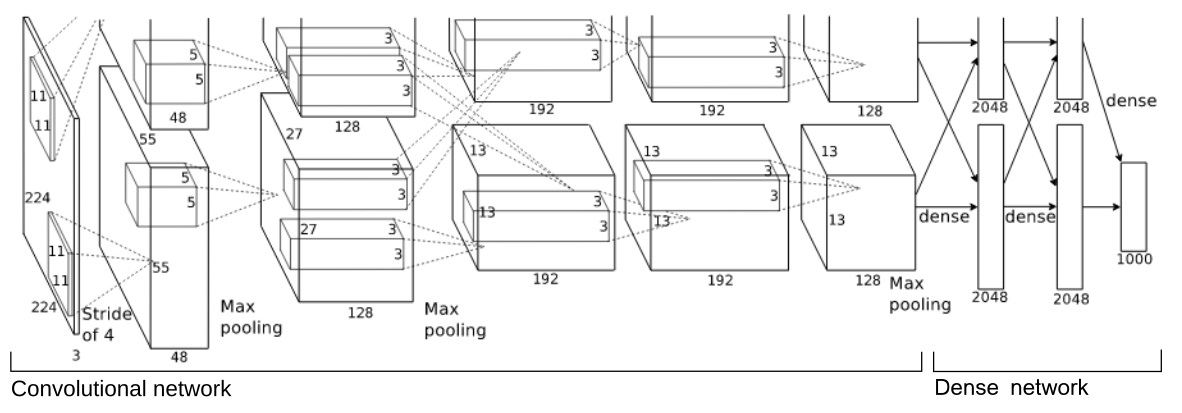
\includegraphics[width=\linewidth]{imagenet-arch}
  }
\end{figure}

Esta arquitectura usa en su primera parte una red convolucional preentrenada sobre un conjunto de imágenes mucho más generalista, en este caso Imagenet. Al usar una red convolucional preentrenada sobre fotografías tendrá muchas más capacidad para distinguir características de diferentes objetos, además que existen varias categorías de peces en Imagenet, por lo que sabrá diferenciar este tipo de fotografías.


\subsection{Red convolucional}

La red convolucional recibir una imagen y devuelve conjunto de i 

\subsection{Modelo preentrenado}

Aqui detallo las implementaciones de los modelos basados en Imagenet (los
disponibles en keras.io): VGG, ResNet e Inception. Tambien tengo que decir
porque prefiero VGG a otros modelos, sobre todo a nivel didactico.

\subsection{Fine tuning}
